\section{Teorema de Cauchy}

El teorema de Cauchy (o integral de Cauchy) es considerado el teorema fundamental de la integración compleja. El enunciado del teorema usa implícitamente el teorema de la curva de Jordan, que establece que una curva continua, simple y cerrada en el plano separa al plano en dos conjuntos abiertos. Uno de estos conjuntos es no acotado y se llama el \textit{exterior}, y el otro es acotado y se llama el \textit{interior}. La curva misma no pertenece a ninguno de estos conjuntos, pero marca la frontera de ambos.

\begin{figure}[ht]
  \centering
  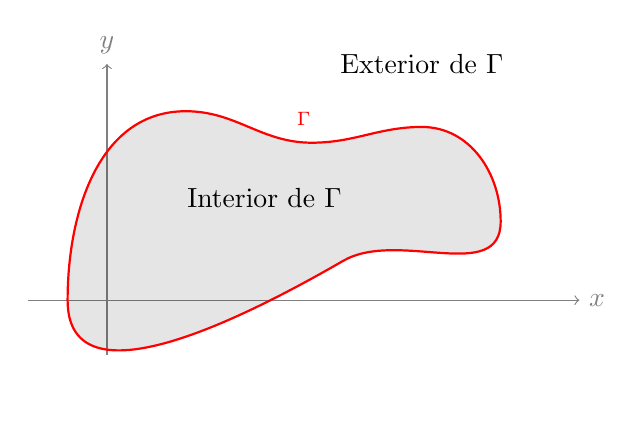
\begin{tikzpicture}
    \draw[->,gray] (-1,0) -- (6,0) node[right] {$x$};
    \draw[->,gray] (0,-0.7) -- (0,3) node[above] {$y$};

    \draw[thick,red,fill=black,fill opacity=0.1] (-0.5,0) to [out=90,in=180] (1,2.4)
    to [out=0,in=180] (2.6,2) 
    to [out=0,in=180] (4,2.2)
    to [out=0,in=90] (5,1)
    to [out=-90,in=30] (3,0.5)
    to [out=210,in=-90] (-0.5,0);
    \node[red] at (2.5,2.3) {\scriptsize$\Gamma$};

    \node at (2,1.3) {Interior de $\Gamma$};
    \node at (4,3) {Exterior de $\Gamma$};
  \end{tikzpicture}
  \caption{Teorema de la curva de Jordan.}
\end{figure}

A pesar de que esta conclusión puede parecer obvia para las curvas cerradas que se suelen dibujar, es difícil de probar debido a la generalidad de su enunciado. 

En la sección \ref{sec:1_curvas_y_regiones_en_el_plano_complejo} estuvimos analizando algunas regiones del plano complejo y sus propiedades. Esto lo hicimos para poder definir el dominio de una función compleja. Ahora vamos a profundizar algunos aspectos sobre las regiones del plano complejo para poder enunciar correctamente el teorema de Cauchy.

\begin{definition}[Trayectoria]
  Una trayectoria es una curva simple, suave a trozos. Una trayectoria pertenece a un conjunto $S$ si su gráfica está contenida dentro de $S$
\end{definition}

Algunas de las curvas paramétricas que hemos realizado anteriormente (como la figura \ref{fig:ejemplo_parabola_gamma}) son trayectorias en $\mathbb{C}$. Así, una trayectoria es una concatenación de curvas suaves que no se cruzan a sí mismas.

\begin{definition}[Conjunto conexo]
  Un conjunto $S$ de números complejos es conexo si, dados dos puntos cualesquiera de $z$ y $w$ en $S$, existe una trayectoria en $S$ que tiene a $z$ y a $w$ como puntos extremos.
\end{definition}

$S$ es conexo si es posible ir desde cualquier punto de $S$ a cualquier otro punto moviéndose a lo largo de alguna trayectoria totalmente contenida en $S$. Un disco abierto es conexo, así como también lo es un disco cerrado (ver sección \ref{sec:1_curvas_y_regiones_en_el_plano_complejo}).

\begin{definition}[Dominio]
  Como ya hemos visto, un conjunto de números complejos, abierto y conexo se llama dominio.
\end{definition}

\begin{definition}[Simplemente conexo]
  Un conjunto $S$ de números complejos es simplemente conexo si toda trayectoria cerrada en $S$ encierra únicamente puntos de $S$.
\end{definition}

Todo disco abierto es simplemente conexo. Si dibuja una trayectoria cerrada en un disco abierto, esta trayectoria cerrada encerará solamente puntos en el disco abierto. El anillo o corona de la figura \ref{fig:corona_complx} no es simplemente conexo. A pesar de ser conexo, se puede dibujar una trayectoria cerrada contenida en el anillo que encierra puntos que no pertenecen al anillo (son aquellos puntos excluidos por la frontera interna).

Ahora si, estamos listos para enunciar el teorema de Cauchy.

\subsection[Enunciado del teorema]{El teorema de Cauchy}

\begin{theorem}[Teorema de Cauchy]
  Sea $f$ diferenciable en un dominio simplemente conexo $G$. Sea $\Gamma$ una trayectoria cerrada en $G$. Entonces
  \[
    \oint_\Gamma f(z)dz=0
  \]
\end{theorem}
